\section{From two real blocks to two existential tests}
\label{sec:two-blocks}

We now consider a sentence
\[
 \exists x\in\R^r\ \forall y\in\R^s\;\Phi(x,y)
\]
in the input model of Theorem~\ref{thm:main}.  The existential decision
procedure already proved does not by itself permit quantification over
the first real block.  We will replace that block by a discrete tuple
of polynomial total bit length.  The main geometric step is to show that, if
some parameter $x$ satisfies the universal condition, then one such
parameter has coordinates singled out by short root labels.

\subsection{Empty fibers and a growing minimum}

First encode failure of the universal condition by a single polynomial.
The encoding must work for every fixed $x$, because $x$ remains a
parameter throughout the construction.

\begin{lemma}[Fiberwise quartic encoding]\label{lem:quartic-fibers}
From a well-formed input of length $N$, one can construct in polynomial
time an explicitly listed polynomial
$F\in\Z[x_1,\ldots,x_r,z_1,\ldots,z_n]$, with $n\ge1$ polynomially
bounded in $N$, such that $F\ge0$ on real inputs, $\deg F\le4$, and,
for every $x\in\R^r$,
\begin{equation}\label{eq:fiber-encoding}
 \exists y\in\R^s\;\neg\Phi(x,y)
 \quad\Longleftrightarrow\quad
 \exists z\in\R^n\;F(x,z)=0.
\end{equation}
The monomial count and coefficient bit lengths of $F$ are polynomially
bounded in $N$.
\end{lemma}

\begin{proof}
Introduce variables for the arithmetic wires in $\Phi$, retaining the
original $x$ variables as parameters.  Each arithmetic gate is enforced
by an equation of degree at most two.  Introduce Boolean value variables
$b$ with $b^2=b$, use the equations
\[
 b=b_1b_2,\qquad b=b_1+b_2-b_1b_2,\qquad b=1-b_1
\]
for AND, OR, and NOT, respectively, and require the output of
$\neg\Phi$ to be $1$.

To couple an atom with polynomial wire value $v$ to its Boolean value
$b$, use fresh real variables $a,a'$ and impose
\begin{align*}
 v=0:\quad &bv=0, & (1-b)(va-1)&=0,\\
 v>0:\quad &b(va^2-1)=0, & (1-b)(v+(a')^2)&=0.
\end{align*}
For an equality atom, $b=0$ is possible exactly when $v\ne0$.
For a positivity atom, $b=1$ is possible exactly when $v>0$, and
$b=0$ exactly when $v\le0$.  Conversely, inverses and real square roots
provide the required witnesses in each of these cases.  Split products
with additional wire variables until every equation has degree at most
two.  The sum of the squares of their left sides is $F$.  Its zeros are
precisely the simultaneous solutions of these equations, proving
\eqref{eq:fiber-encoding} for each fixed $x$.

There are polynomially many bounded-size equations, with polynomial
coefficient bit lengths.  Expanding their squares therefore gives the
asserted monomial list.  The variables $z$ include $y$ and all auxiliary
variables; an unused variable ensures $n\ge1$ if necessary.
\end{proof}

Call $x$ \emph{good} if $F(x,\cdot)$ has no real zero.  By
Lemma~\ref{lem:quartic-fibers}, our task is to decide whether a good
parameter exists.  Introduce a nonnegative real parameter $u$ and set
\begin{equation}\label{eq:fiber-minimum}
 h(x,u,z)=\sum_{i=1}^n z_i^6+6uF(x,z),
 \qquad
 m_x(u)=\min_{z\in\R^n}h(x,u,z).
\end{equation}
The coercive term prevents minimizers from escaping whenever their
values remain bounded.  In particular, the minimum exists and is
nonnegative.  For fixed $x$ it is nondecreasing in $u$.

The function $(x,u)\mapsto m_x(u)$ is continuous on
$\R^r\times[0,\infty)$.  Indeed, on a compact parameter neighborhood,
comparison with $z=0$ gives a uniform upper bound on the minimum.
Since $h(x,u,z)\ge\sum_i z_i^6$, all minimizers lie in one compact set.
Uniform continuity of $h$ on that set and the parameter neighborhood
then implies continuity of its minimum.  Moreover,
\begin{equation}\label{eq:good-divergence}
 x\text{ is good}
 \quad\Longleftrightarrow\quad
 m_x(u)\longrightarrow+\infty\quad(u\longrightarrow+\infty).
\end{equation}
A zero of $F(x,\cdot)$ supplies a uniform upper bound.  Conversely, if
the nondecreasing minimum stays bounded, take minimizers along
$u\to+\infty$.  They stay in a compact set, and
$6uF(x,z)\le h(x,u,z)$ forces $F(x,z)\to0$ along them.
A limit point is a zero of the fiber polynomial.

At each minimizer the critical equations are
\[
 f_i=z_i^5+u\frac{\partial F}{\partial z_i}=0
 \qquad(1\le i\le n).
\]
Their lower-degree terms have $z$-degree at most $3$.
Proposition~\ref{prop:multiplication-determinant}, with $x,u$ as
parameters, therefore constructs a controlled polynomial
\begin{equation}\label{eq:fiber-characteristic}
 Q(x,u,T)=\det(TI-M_h),\qquad D=5^n.
\end{equation}
It is monic of degree $D$ in $T$, and evaluation at a critical point
gives
\begin{equation}\label{eq:minimum-root}
 Q(x,u,m_x(u))=0.
\end{equation}
We next use this one polynomial to separate the parameters with bounded
minima from those with divergent minima.

\subsection{Degree pieces and a closed lift}

The rate of divergence in \eqref{eq:good-divergence} can be detected by
a fixed power substitution.  For each fixed $x$,
\begin{equation}\label{eq:growth-test}
 \begin{cases}
 m_x(v^{D+1})>v\text{ for all sufficiently large }v,&x\text{ good},\\
 m_x(v^{D+1})<v\text{ for all sufficiently large }v,&x\text{ not good}.
 \end{cases}
\end{equation}
The second assertion follows from boundedness.  For the first, write
the specialization of $Q$ at $x$ as
\[
 Q(x,u,T)=\sum_{j=0}^a q_j(T)u^j,\qquad q_a\ne0,
 \qquad\deg q_j\le D.
\]
If a sequence $v\to+\infty$ satisfied $m_x(v^{D+1})\le v$, put
$t_v=m_x(v^{D+1})$.  Then $t_v\to+\infty$, whereas
\eqref{eq:minimum-root}, divided by $v^{a(D+1)}$, gives
\[
 q_a(t_v)=-\sum_{j<a}q_j(t_v)v^{-(a-j)(D+1)}\longrightarrow0.
\]
Here $0\le t_v\le v$ makes each term on the right $O(v^{-1})$.
A nonzero polynomial cannot tend to zero along a sequence tending to
$+\infty$, giving the contradiction.

To control the growth test locally as $x$ varies, we track possible
zeros of $m_x(v^{D+1})-v$.  By \eqref{eq:minimum-root}, each such
zero forces $Q(x,v^{D+1},v)=0$.  Define the controlled polynomial
\begin{equation}\label{eq:degree-polynomial}
 E(x,v)=Q(x,v^{D+1},v)=\sum_{j=0}^{d_E}E_j(x)v^j,
\end{equation}
where $d_E$ is a short, polynomial-time computable degree bound.
Coefficient extraction makes the $E_j$ a uniformly controlled family.
Crucially,
\begin{equation}\label{eq:nonzero-degree-polynomial}
 E_D(x)=1\qquad\text{for every }x.
\end{equation}
Indeed, the term $T^D$ in $Q$ gives $v^D$.  Every other term has
$T$-degree at most $D-1$, so after substitution its $v$-exponent has
the form $a(D+1)+b$ with $a\ge0$ and $0\le b<D$; none equals $D$.
Thus $E(x,\cdot)$ is never the zero polynomial.
Fixing its actual degree keeps its leading coefficient locally away
from zero, and hence gives a locally uniform bound on its roots.

\begin{proposition}[Local constancy on degree pieces]
\label{prop:degree-pieces}
For $0\le d\le d_E$, let
\[
 A_d=\{x\in\R^r:E_d(x)\ne0,\ E_j(x)=0\text{ for }j>d\}.
\]
The sets $A_d$ partition $\R^r$.  Within each $A_d$, the good
parameters form a subset that is both open and closed in the relative
topology.
\end{proposition}

\begin{proof}
The partition assertion follows from
\eqref{eq:nonzero-degree-polynomial}.  Fix $x_0\in A_d$.
On a neighborhood $V$ of $x_0$ relative to $A_d$, continuity bounds
$|E_d|$ below by a positive number and all the other coefficient
moduli above.  The elementary leading-term bound therefore gives
$R>0$ such that
\[
 E(x,v)\ne0\qquad(x\in V,\ v\ge R).
\]
Consequently the continuous function
$m_x(v^{D+1})-v$ never vanishes on this range: a zero would contradict
\eqref{eq:minimum-root} and \eqref{eq:degree-polynomial}.
For each $x\in V$ its sign is constant as $v$ varies in $[R,\infty)$,
and \eqref{eq:growth-test} identifies that sign with goodness.
By continuity in $x$, its nonzero sign at $v=R$ is constant on a
smaller relative neighborhood of $x_0$.  Goodness is therefore locally
constant on $A_d$, which proves both relative openness and relative
closedness.
\end{proof}

The sets $A_d$ need not be closed in the ambient space.  To make the
separation in Proposition~\ref{prop:degree-pieces} usable in a compact
minimization argument, introduce one real variable $t$ and define
\begin{equation}\label{eq:closed-lift}
 W_d(x,t)=(E_d(x)t-1)^2+\sum_{j=d+1}^{d_E}E_j(x)^2,
 \qquad
 Z_d=\{(x,t)\in\R^{r+1}:W_d(x,t)=0\}.
\end{equation}
The $W_d$ are nonnegative controlled polynomials, uniformly in the short
index $d$.  The set $Z_d$ is closed, and projection onto $x$ is a
homeomorphism from $Z_d$ onto $A_d$, with inverse
$x\mapsto(x,1/E_d(x))$.  Thus the good part of $Z_d$ and its
complement in $Z_d$ are both closed in the ambient Euclidean space.
We have separated the two behaviors without needing a description of
the connected components of a degree piece.

\subsection{Algebraic coordinates in a selected closed part}

We now show that a nonnegative polynomial $W$ supplies coordinate
polynomials whose roots include the coordinates of a point in every
nonempty part of $\{W=0\}$ that is both open and closed within that
zero set.  Their construction is independent of which part is selected
and requires no equations describing that part.
The use of a deformation and limiting characteristic-polynomial roots
is related to the sampling methods in
Basu, Pollack, and Roy~\cite[Sections~12.5--12.6]{BasuPollackRoy2006}.
The argument below proves the precise form needed here directly.

\begin{proposition}[Candidate coordinates]
\label{prop:candidate-coordinates}
Let $W\in\R[c_1,\ldots,c_k]$ be nonnegative on $\R^k$, where $k\ge1$,
and let $C$ be a nonempty subset of $Z=\{W=0\}$ that is both open and
closed in $Z$.  Choose an odd integer $\ell\ge3$ with $\ell>\deg W$,
and put
\[
 G(c)=\sum_{i=1}^k c_i^{\ell+1},\qquad
 H_w(c)=G(c)+(\ell+1)wW(c).
\]
In the quotient by
\begin{equation}\label{eq:candidate-relations}
 c_i^\ell+w\frac{\partial W}{\partial c_i}=0
 \qquad(1\le i\le k),
\end{equation}
form the coordinate multiplication polynomials
\begin{equation}\label{eq:coordinate-polynomials}
 P_i(w,T)=\det(TI-M_{c_i})=\sum_j P_{i,j}(T)w^j.
\end{equation}
For each $i$, let $j_i$ be the largest index for which
$P_{i,j_i}\ne0$.  There exists $c^*\in C$ such that
\[
 P_{i,j_i}(c_i^*)=0\qquad(1\le i\le k).
\]
If $W$ is a controlled family of integer polynomials, $k$ is
polynomially bounded, and $\ell$ is short and computable in polynomial
time, then the polynomials $P_i$ and $P_{i,j}$ are uniformly controlled.
\end{proposition}

\begin{proof}
The relations \eqref{eq:candidate-relations} satisfy the degree
hypotheses of Lemma~\ref{lem:monomial-basis}, with coefficient ring
$\R[w]$.  Thus the coordinate multiplication matrices exist, and each
$P_i$ is monic of degree $\ell^k$ in $T$.  In particular, $P_i\ne0$
and $j_i$ exists.  For controlled integer families,
Proposition~\ref{prop:multiplication-determinant} and coefficient
extraction give the final assertion.

Fix $c^0\in C$ and choose $M>G(c^0)$.  The set
\[
 K_0=\{c:G(c)\le M\}
\]
is compact.  Since $Z$ is closed and $C$ is relatively both open and
closed, the sets
\[
 S_g=C\cap K_0,\qquad S_b=(Z\setminus C)\cap K_0
\]
are disjoint compact sets, and $c^0\in S_g$.  Choose $\epsilon>0$
so that the compact set
\begin{equation}\label{eq:compact-neighborhood}
 K=\{c\in K_0:\operatorname{dist}(c,S_g)\le\epsilon\}
\end{equation}
is disjoint from $S_b$.  This is possible because disjoint nonempty
compact sets have positive distance; if $S_b$ is empty, any positive
$\epsilon$ suffices.  Figure~\ref{fig:compact-neighborhood} indicates
the two boundaries whose role we must control.

For a sequence $w_\nu>0$ tending to $+\infty$, let $c^\nu$ minimize
$H_{w_\nu}$ on $K$.  Since $c^0\in K$ and $W(c^0)=0$, nonnegativity
gives
\begin{equation}\label{eq:penalty-bounds}
 G(c^\nu)+(\ell+1)w_\nu W(c^\nu)
 \le G(c^0)<M.
\end{equation}
After passage to a subsequence, compactness gives $c^\nu\to c^*\in K$.
The same bound forces $W(c^\nu)\to0$, so $c^*\in Z\cap K$.
Because $K\cap S_b=\varnothing$, we have $c^*\in S_g\subset C$.
Furthermore,
\[
 G(c^*)\le G(c^0)<M,
 \qquad \operatorname{dist}(c^*,S_g)=0<\epsilon.
\]
Both inequalities defining $K$ are strict at $c^*$, so $c^*$ is an
interior point of $K$.  Hence the convergent minimizers $c^\nu$ are
also interior for all sufficiently large $\nu$.  They satisfy the
unconstrained critical equations \eqref{eq:candidate-relations}.
Evaluation at these common zeros gives
\[
 P_i(w_\nu,c_i^\nu)=0.
\]
Divide by $w_\nu^{j_i}$.  The lower powers tend to zero because
$c_i^\nu$ stays bounded, and passage to the limit yields
$P_{i,j_i}(c_i^*)=0$, as required.
\end{proof}

\begin{figure}[tb]
\centering
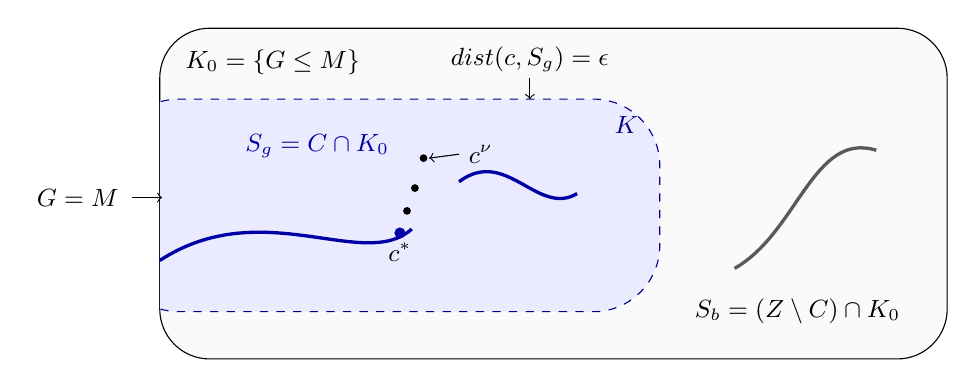
\begin{tikzpicture}[x=1cm,y=1cm, font=\small]
 \draw[rounded corners=18pt,fill=black!2] (0,0) rectangle (10,4.2);
 \node[anchor=north west] at (.2,4.05) {$K_0=\{G\le M\}$};
 \begin{scope}
 \clip[rounded corners=18pt] (0,0) rectangle (10,4.2);
 \draw[rounded corners=24pt,fill=blue!8,draw=blue!55!black,dashed]
   (-.6,.6) rectangle (6.35,3.3);
 \end{scope}
 \node[anchor=north east,text=blue!55!black] at (6.2,3.2) {$K$};
 \draw[very thick,blue!65!black] (0,1.25) .. controls (1.3,2.1)
   and (2.6,1.1) .. (3.2,1.65);
 \draw[very thick,blue!65!black] (3.8,2.25) .. controls (4.4,2.7)
   and (4.8,1.8) .. (5.3,2.1);
 \node[text=blue!65!black] at (2,2.7) {$S_g=C\cap K_0$};
 \node[anchor=east] at (-.4,2.05) {$G=M$};
 \draw[->] (-.35,2.05) -- (.03,2.05);
 \node at (4.7,3.8) {$\operatorname{dist}(c,S_g)=\epsilon$};
 \draw[->] (4.7,3.57) -- (4.7,3.3);
 \draw[very thick,black!65] (7.3,1.15) .. controls (8.1,1.6)
   and (8.3,2.9) .. (9.1,2.65);
 \node[align=center] at (8.1,.6) {$S_b=(Z\setminus C)\cap K_0$};
 \fill[blue!65!black] (3.05,1.6) circle (2pt);
 \node[below] at (3.05,1.6) {$c^*$};
 \fill (3.35,2.55) circle (1.4pt);
 \fill (3.24,2.17) circle (1.4pt);
 \fill (3.14,1.88) circle (1.4pt);
 \draw[->] (3.8,2.6) -- (3.42,2.55);
 \node[anchor=west] at (3.8,2.6) {$c^\nu$};
\end{tikzpicture}
\caption{The compact-neighborhood argument, schematically.  The selected
zero set $S_g$ and the excluded zero set $S_b$ are separated inside
$K_0$.  The set $K$ can meet the boundary $G=M$.  Penalized minimizers
converge to $c^*\in S_g$ with $G(c^*)<M$ and distance zero from $S_g$,
strictly below $\epsilon$.  They are therefore eventually interior to
$K$, away from both boundary portions.  The drawn shapes assert no
smoothness or connectedness of these sets.}
\label{fig:compact-neighborhood}
\end{figure}

Apply Proposition~\ref{prop:candidate-coordinates} to $W=W_d$ and to
the good part of $Z_d$.  We use $c=(x,t)\in\R^{r+1}$ and choose
$\ell$ from a uniform short degree bound on $W_d$.  Whenever this good
part is nonempty, it contains a point whose coordinates are roots of
the nonzero coefficient polynomials $P_{i,j_i}$.  These polynomials
are controlled uniformly in $d,i,j_i$.

\subsection{The final decision}

We can now use root labels to replace the real choice of $x$ by short
discrete data.  Choose an integer $0\le d\le d_E$ and, for each
$1\le i\le r+1$, an index $j_i$ within a uniform short bound on the
$w$-degree of $P_i$.  For each $P_{i,j_i}$ choose root-label data as
in Proposition~\ref{prop:root-labels}, with the auxiliary positivity
test equal to $1$, and write $L_i$ for the resulting controlled
polynomial.  Let $\mathcal S(c)$ denote the conjunction
\begin{equation}\label{eq:selected-coordinates}
 W_d(c)=0,\qquad
 P_{i,j_i}(c_i)=0,\qquad L_i(c_i)>0
 \quad(1\le i\le r+1).
\end{equation}
For these choices, accept exactly when both statements hold:
\begin{align}
 &\exists c\in\R^{r+1}\;\mathcal S(c),
 \label{eq:final-nonempty}\\
 &\neg\exists(c,z)\in\R^{r+1+n}\;
       \bigl(\mathcal S(c)\ \wedge\ F(x,z)=0\bigr).
 \label{eq:final-no-counterexample}
\end{align}
Each existential statement is an instance of
Theorem~\ref{thm:controlled-existential}.  Their conjunction, with
negation as displayed, is therefore an available decision.

We verify the two directions separately; they use the labels in
different ways.  If the test accepts, choose $c=(x,t)$ from
\eqref{eq:final-nonempty}.  Statement
\eqref{eq:final-no-counterexample} implies that $F(x,\cdot)$ has no
real zero.  Thus $x$ is good.  This implication holds for every choice
of the indices and labels, even if a selected coefficient polynomial
is zero or the conjunction selects more than one point.

Conversely, suppose a good $x$ exists.  Let $d$ be the actual degree
of $E(x,\cdot)$.  Then the good part of $Z_d$ is nonempty.
Proposition~\ref{prop:candidate-coordinates} supplies a point
$c^*=(x^*,t^*)$ in that part and highest nonzero coefficient indices
$j_i$ for which $P_{i,j_i}(c_i^*)=0$.  By
Proposition~\ref{prop:root-labels}, labels can be chosen to single out
each $c_i^*$ among the real roots of its coefficient polynomial.
For these choices, \eqref{eq:selected-coordinates} has exactly the
one solution $c^*$.  It satisfies
\eqref{eq:final-nonempty}, and goodness of $x^*$ gives
\eqref{eq:final-no-counterexample}.  Some discrete choices therefore
accept.  Notice that the decision procedure does not need to verify
that an index is highest or a coefficient polynomial nonzero: those
properties provide complete choices, whereas the two tests ensure
soundness for all choices.

Finally, all discrete choices together have polynomial encoding length.
There are only $r+1$ coefficient indices and labels; each degree bound,
index bound, and label bound is short.  The real variables and the
number of equations and positivity tests in
\eqref{eq:final-nonempty}--\eqref{eq:final-no-counterexample} are
polynomially bounded.  The controlled-polynomial rules are used in a
fixed order: construct $Q$ and $E$, extract their coefficients and form
$W_d$, construct the coordinate polynomials, form the labels, and apply
the two existential tests.  Each stage is uniform in its short indices;
none introduces a separate oracle or one counting level per index.
The existential quantification over the entire discrete choice tuple
thus preserves availability.  The resulting decision function belongs
to a fixed level of the counting hierarchy, independent of the input.
Malformed inputs were rejected in polynomial time, so this proves
Theorem~\ref{thm:main}.
